\chapter{Rezultate teoretice și experimentale}
\label{cap:rezultate}

În cadrul acestui capitol vor fi prezentate o serie de rezultate prin care poate fi analizată eficiența metodei propuse în cadrul capitolui\ref{cap:contributii}.

\section{Analiza strategiilor de selecție a lanțurilor de tipare închise}

Pentru rezultate prezentate în cadrul următoarelor tabele s-au folosit jumătate dintre cuvintele silabisite din setul de date RoSyllabiDict ($\sim200.000$) pentru identficarea de tipare frecvente. 

Pentru validarea strategiilor s-au extras aleatoriu, 10.000 de cuvinte din a doua jumătate a setului de cuvinte RoSyllabiDict.

În cazul strategiei care selectează silabisirea idenficată cu cele mai multe lanțuri de tipare inchise, rezultate sunt ilustrate în cadrul tabelului ~\ref{table:counting}.

\begin{table}[h!]
\centering
\begin{tabular}{|c|c|c|c|c|}
\hline
suport minim & $m_d$ & $\sum m_w$ & $\%{m_w}$ & cuvinte nedespărțite\\ 
\hline
\hline
50 & 0.898810282887619 & 4719 & 51.85 & 899\\ 
\hline
45 & 0.895689133288429 & 4644 & 50.53 & 810\\ 
\hline
40 & 0.893229396558503 & 4665 & 50.28 & 722\\ 
\hline
35 & 0.89376043637831 & 4740 & 50.68 & 648\\ 
\hline
30 & 0.890320159357963 & 4681 & 49.55 & 553\\ 
\hline
25 & 0.889120134369591 & 4713 & 49.4 & 459\\ 
\hline
20 & 0.888821085026373 & 4808 & 49.85 & 355\\ 
\hline
15 & 0.886419928605455 & 4773 & 49 & 260\\ 
\hline
10 & 0.875989677334146 & 4210 & 42.84 & 173\\ 
\hline
5 & 0.859792028980429 & 3672 & 37.01 & 78\\ 
\hline\end{tabular}
\caption{Evaluarea strategiei bazată pe numarul de lanțuri de tipare închise echivalente} 
\label{table:counting}
\end{table}

În cadrul tabelei ~\ref{table:overlapping} sunt ilustrate rezultate analizei în cazul strategiei bazată pe suprapuneri. 

\begin{table}[h!]
\centering
\begin{tabular}{|c|c|c|c|c|}
\hline
suport minim & $m_d$ & $\sum m_w$ & $\%{m_w}$ & cuvinte nedespărțite\\ 
\hline
\hline
50 & 0.934182795192563 & 5669 & 62.29 & 899\\ 
\hline
45 & 0.933385818781609 & 5698 & 62 & 810\\ 
\hline
40 & 0.935090134710169 & 5830 & 62.84 & 722\\ 
\hline
35 & 0.935032634560768 & 5908 & 63.17 & 648\\ 
\hline
30 & 0.934206185385081 & 5933 & 62.8 & 553\\ 
\hline
25 & 0.935714036164661 & 6036 & 63.26 & 459\\ 
\hline
20 & 0.934152429276784 & 6076 & 63 & 355\\ 
\hline
15 & 0.936083160365696 & 6211 & 63.77 & 260\\ 
\hline
10 & 0.936303244543237 & 6269 & 63.79 & 173\\ 
\hline
5 & 0.928531534060846 & 5916 & 59.63 & 78\\ 
\hline\end{tabular}
\caption{Evaluarea strategiei bazate pe nivelul de suprapunere} 
\label{table:overlapping}
\end{table}

Iar în cadrul tabelei ~\ref{table:shortest} este ilustrată evaluarea strategiei bazate pe lungimea lanțurilor de tipare închise.

\begin{table}[h!]
\centering
\begin{tabular}{|c|c|c|c|c|}
\hline
suport minim & $m_d$ & $\sum m_w$ & $\%{m_w}$ & cuvinte nedespărțite\\  
\hline
\hline
50 & 0.948261855927185 & 6392 & 70.23 & 899\\ 
\hline
45 & 0.947471781784847 & 6458 & 70.27 & 810\\ 
\hline
40 & 0.948916493018081 & 6588 & 71.01 & 722\\ 
\hline
35 & 0.950700978994344 & 6727 & 71.93 & 648\\ 
\hline
30 & 0.950471973129913 & 6820 & 72.19 & 553\\ 
\hline
25 & 0.952801443394629 & 6985 & 73.21 & 459\\ 
\hline
20 & 0.954658800101994 & 7171 & 74.35 & 355\\ 
\hline
15 & 0.956975673054947 & 7337 & 75.33 & 260\\ 
\hline
10 & 0.959539699499725 & 7500 & 76.32 & 173\\ 
\hline
5 & 0.958024515826585 & 7633 & 76.93 & 78\\ 
\hline\end{tabular}
\caption{Evaluarea strategiei bazate pe lungimea lanțurilor de tipare închise} 
\label{table:shortest}
\end{table}

La nivel comparativ, în cadrul figurilor ~\ref{fig:strategies-word} și \ref{fig:strategies-point} se poate observa evoluția preciziei la nivelul ambelor metrici definite anterior. 


\begin{figure}[h!]
    \centering
    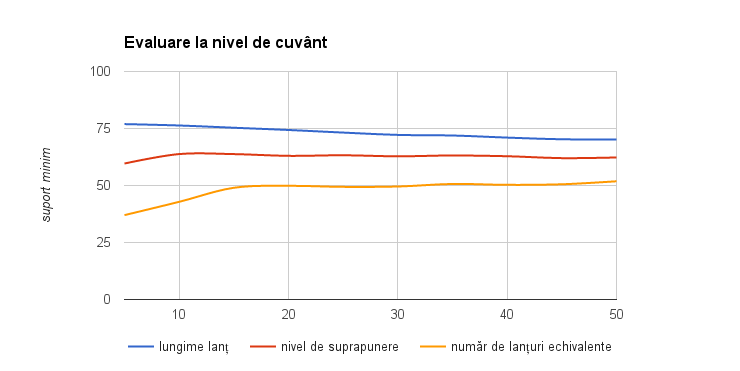
\includegraphics[width=1\textwidth]{figures/strategies-word.png}
    \caption{Evaluare comparativă a strategiilor ($\%m_w$)}
    \label{fig:strategies-word}
\end{figure}


\begin{figure}[h!]
    \centering
    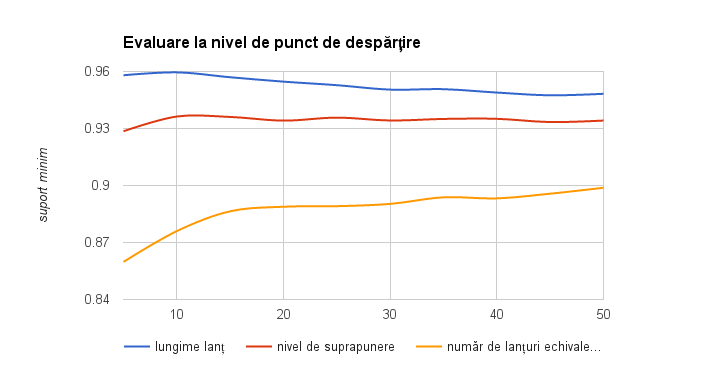
\includegraphics[width=1\textwidth]{figures/strategies-point.png}
    \caption{Evaluare comparativă a strategiilor ($m_d$)}
    \label{fig:strategies-point}
\end{figure}

Din cele două figuri putem trage două concluzii:

\begin{itemize}
\item strategia bazată pe lungimea lanțului de tipare închis performează cel mai bine. 
\item cele două metrici reflectă aleasi rezultate. 
\end{itemize}

\section{Analiza comparativă cu alte metode de silabisire}

Pentru a încadra rezultatele relativ la alte abordări, au fost preluate rezultate din cadrul articolului ~\cite{bib:dinu2013romanian} și sunt prezentate în cadrul tabelei ~\ref{table:comparison}. 

Trebuie menționat că deși metoda prezentată în cadrul acestei lucrări, nu excelează la precizie, aceasta prezintă un nivel ridicat de genericitate. în cadrul tabelului 

\begin{table}[t!]
\centering
\begin{tabular}{|c|c|c|c|c|}
\hline
Abordare & Acuratețe la nivel de cuvânt\\  
\hline
\hline
RULE & 60,67\%\\ 
\hline
\color{cyan} FSP & \color{cyan}76,93\% \\ 
\hline
SVM & 90,46\%\\ 
\hline
CRF & 95,25\%\\ 
\hline\end{tabular}
\caption{Evaluare comparativă cu alte soluții} 
\label{table:comparison}
\end{table}
